% master.tex
% Copyright 2016 Zheng Xie <xie.zheng777@gmail.com>
% https://github.com/Tedxz/xjtuthesis-x
%
% This work may be distributed and/or modified under the
% conditions of the LaTeX Project Public License, either version 1.3
% of this license or (at your option) any later version.
% The latest version of this license is in
%   http://www.latex-project.org/lppl.txt
% and version 1.3 or later is part of all distributions of LaTeX
% version 2005/12/01 or later.
%
% This work has the LPPL maintenance status `maintained'.
%
% The Current Maintainer of this work is Zheng Xie.
%
% xjtuthesis-x is a Derived Work of xjtuthesis. The original maintainer of
% xjtuthesis is Weisi Dai (multiple1902 <multiple1902@gmail.com>),
% who published the project on https://code.google.com/p/xjtuthesis/ (no
% longer accessable). Currently, xjtuthesis is maintained by Aetf, and can
% be accessed on https://github.com/Aetf/xjtuthesis.
%
% xjtuthesis-x includes bug fixes, new features and a user guide.
% For detail, please refer to Readme.md.
%
% If you want to contribute to xjtuthesis-x or become the maintainer of
% xjtuthesis-x, please feel free to contact me.

\documentclass[
    master,
    truefont, % just turn it on when using Windows
    %nofont, % remember to manally set the fonts
    pdflinks,
    %colorlinks,
    %compact,
    ]{xjtuthesis}
% \usepackage[UTF8]{ctex}
% \usepackage[utf8]{inputenc}
\usepackage{etoolbox}
\usepackage{fmtcount}
\usepackage{overpic}
\usepackage{lmodern}

\preto{\section}{\setcounter{subsubsection}{0}}
\graphicspath{{figures/}}
\addbibresource{bibliography.bib}
\begin{document}
    \setmainfont{Times New Roman}
    % 请修改 meta.tex 中的论文元信息
    % meta.tex
% Copyright 2016 Zheng Xie <xie.zheng777@gmail.com>
% https://github.com/Tedxz/xjtuthesis-x
%
% This work may be distributed and/or modified under the
% conditions of the LaTeX Project Public License, either version 1.3
% of this license or (at your option) any later version.
% The latest version of this license is in
%   http://www.latex-project.org/lppl.txt
% and version 1.3 or later is part of all distributions of LaTeX
% version 2005/12/01 or later.
%
% This work has the LPPL maintenance status `maintained'.
%
% The Current Maintainer of this work is Zheng Xie.
%
% xjtuthesis-x is a Derived Work of xjtuthesis. The original maintainer of
% xjtuthesis is Weisi Dai (multiple1902 <multiple1902@gmail.com>),
% who published the project on https://code.google.com/p/xjtuthesis/ (no
% longer accessable). Currently, xjtuthesis is maintained by Aetf, and can
% be accessed on https://github.com/Aetf/xjtuthesis.
%
% xjtuthesis-x includes bug fixes, new features and a user guide.
% For detail, please refer to Readme.md.
%
% If you want to contribute to xjtuthesis-x or become the maintainer of
% xjtuthesis-x, please feel free to contact me.

% 标题,中文
\ctitle{XXXXXXXXXXXXXXXXXXXXXXXXXXXXXXX}

% 作者,中文
\cauthor{XXX}

% 学科,中文,本科生不需要
\csubject{控制科学与工程}

% 导师姓名,中文
\csupervisor{XXX~教授}

% 关键词,中文。用全角分号「;」分割
% 研究生的应首先从《汉语主题词表》中摘选
\ckeywords{XXX;XXX;XXX;XXX;XXX}

% 提交日期,本科生不需要
\cproddate{\the\year 年\the\month 月}

% 论文类型,中文,本科生不需要
% 从理论研究、应用基础、应用研究、研究报告、软件开发、设计报告、案例分析、调研报告、其它中选择
\ctype{应用研究}

% 论文标题,英文
\etitle{XXXXXXXXXXXXXXXXXXXXXXXXXXXXXXXXx}

% 作者姓名,英文
\eauthor{Xxsheng Xxxx}

% 学科,英文,本科生不需要
\esubject{Control Science and Engineering}

% 导师姓名,英文
\esupervisor{Prof. Xxxxsheng Zzzz}

% 关键词,英文。用半角分号和一个半角空格「; 」分割
\ekeywords{XXX;XXX; XXX; XXX; XXX}

% 学科门类,英文
% 从Philosophy(哲学)、Economics(经济学)、Law(法学)、Education(教育学)、Arts(文学)、
%   Science(理学)、Engineering Science(工学)、Medicine(医学)、Management Science(管理学)中选择
\ecate{Engineering Science}

% 提交日期,英文,本科生不需要
% 应当和 cproddate 保持一致
\eproddate{\monthname{\month}\ \the\year}

% 论文类型,英文,本科生不需要
% 从Theoretical Research(理论研究)、Application Fundamentals(应用基础)、Applied Research(应用研究)、
%   Research Report(研究报告)、Software Development(软件开发)、Design Report(设计报告)、
%   Case Study(案例分析)、Investigation Report(调研报告)、其它(Other)中选择
\etype{Applied Research}

% 摘要,中文。段间空行
\cabstract{
我是摘要,我主要完成了以下工作:
\begin{itemize}
    \item[1)] XXX。

    \item[2)] YYY。

    \item[3)] ZZZ。
    
\end{itemize}
    

}

% 摘要,英文。段间空行
\eabstract{
    I am abstract. The work of this thesis are summarized as follows:
    \begin{itemize}
        \item[1)] XXX.

        \item[2)] YYY.
        
        \item[3)] ZZZ.
\end{itemize}

}


    \xjtuchead
    \xjtuehead

    \xjtudabianweiyuanhui % 请在xjtuthesis.cls中修改您的答辩人信息。
    % 以pdf的形式插入答辩人信息
    % {
    %     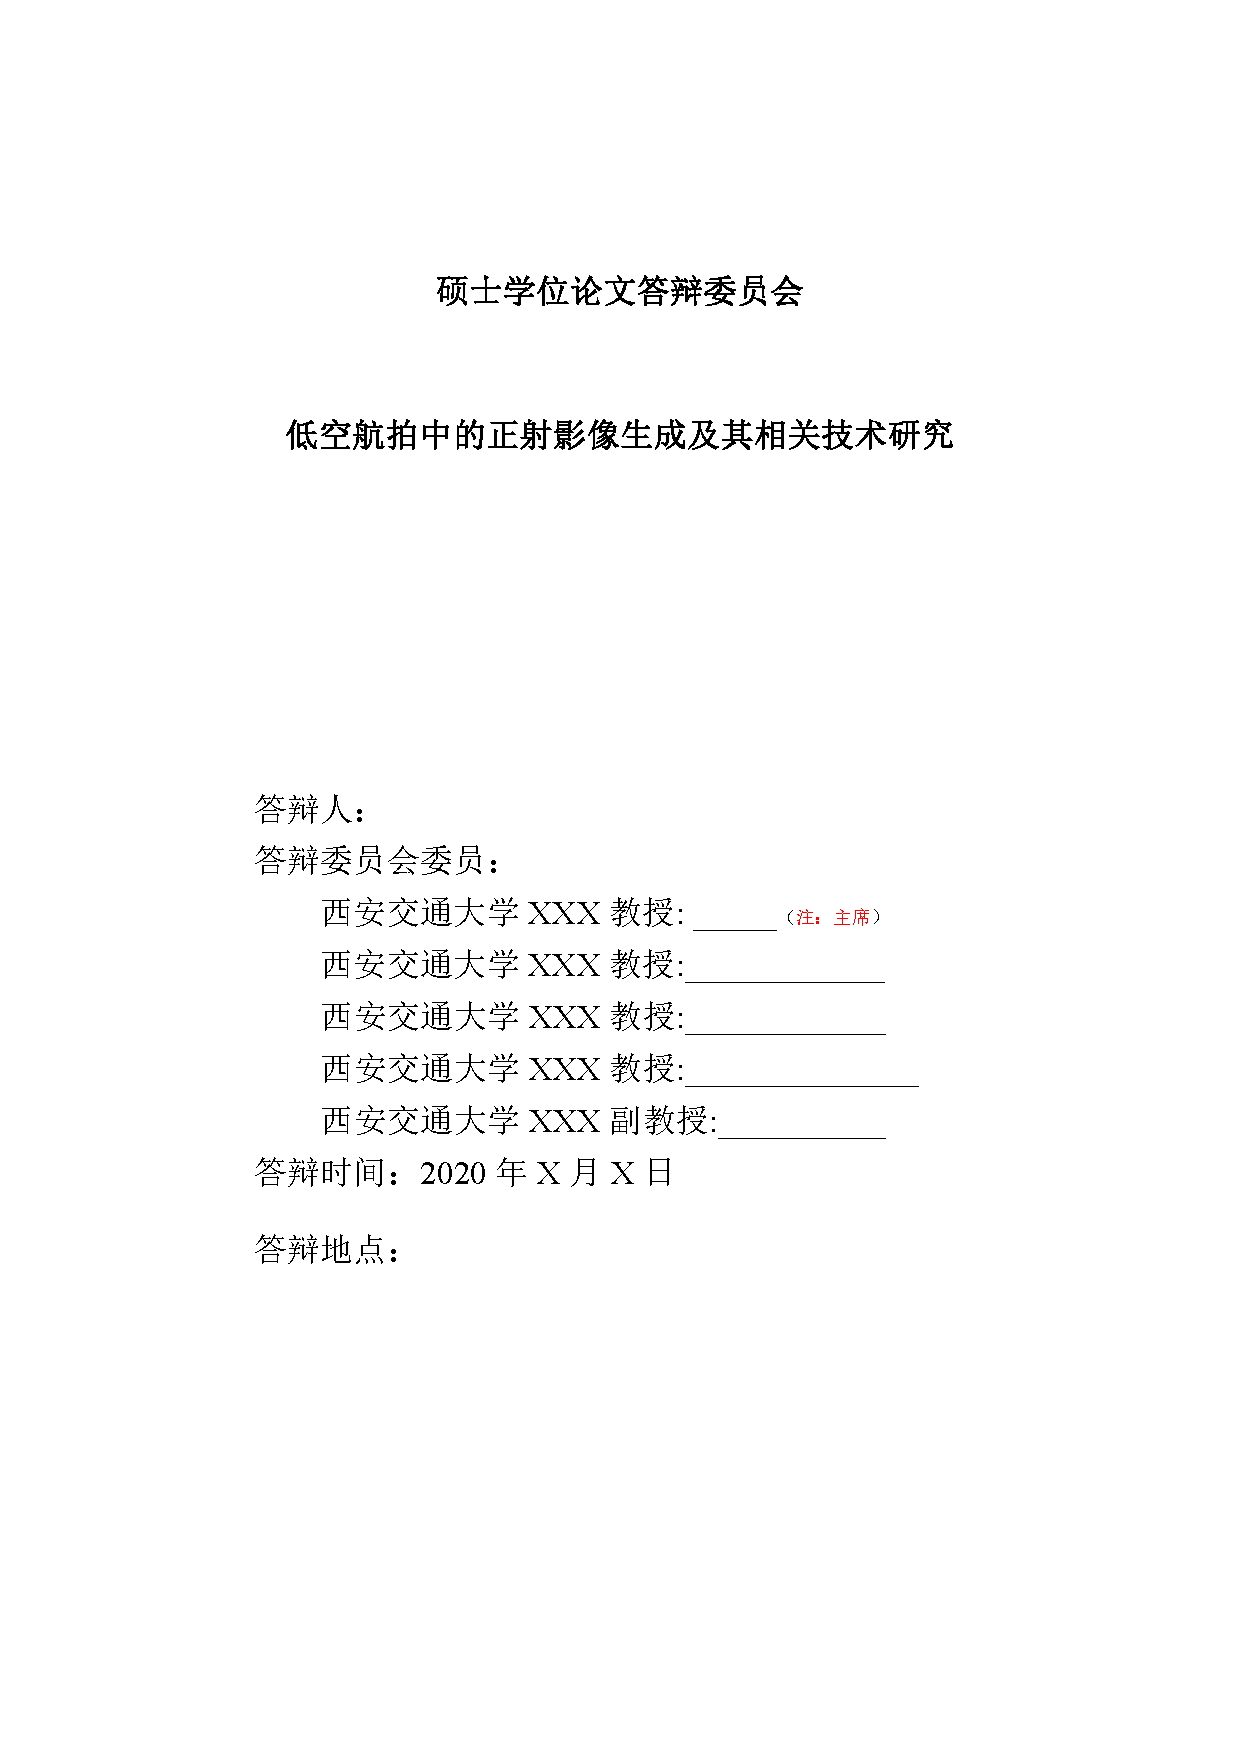
\includepdf[pages={1}]{figures/答辩委员会.pdf}
    %     \thispagestyle{empty}
    %     \cleardoublepage
    % }

    \xjtucinfopage
    \xjtueinfopage
    \xjtutoc
    \xjtutoe
    \clearpage

    % multiple1902 <multiple1902@gmail.com>
% denotation.tex
% Copyright 2011~2012, multiple1902 (Weisi Dai)
% https://code.google.com/p/xjtuthesis/
% 
% It is strongly recommended that you read documentations located at
%   http://code.google.com/p/xjtuthesis/wiki/Landing?tm=6
% in advance of your compilation if you have not read them before.
%
% This work may be distributed and/or modified under the
% conditions of the LaTeX Project Public License, either version 1.3
% of this license or (at your option) any later version.
% The latest version of this license is in
%   http://www.latex-project.org/lppl.txt
% and version 1.3 or later is part of all distributions of LaTeX
% version 2005/12/01 or later.
%
% This work has the LPPL maintenance status `maintained'.
% 
% The Current Maintainer of this work is Weisi Dai.
%
\begin{denotation}
        \item[符号1]    解释1
        \item[符号2]    解释2
\end{denotation}
如果论文中使用了大量的物理量符号、标志、缩略词、专门计量单位、自定义名词和术语等,应将全文中常用的这些符号及意义列出。如果上述符号和缩略词使用数量不多,可以不设专门的主要符号表,但在论文中出现时须加以说明。
论文中主要符号应全部采用法定单位,特别要严格执行GB3100~3102—93有关“量和单位”的规定。单位名称的书写,可以采用国际通用符号,也可以用中文名称,但全文应统一,不得两种混用。
缩略词应列出中英文全称。
主要符号表正文统一左缩进一个字符。
符号表排序方法:先按拉丁字母大写、小写排序,再按希腊字母大写、小写排序。
部分内容非强制性要求,如果论文中所用符号不多,可以省略《主要符号表》 % 主要符号表可选

    \xjtucontent
        \chapter{绪论}
\echapter{Preface}
\section{研究背景与意义}
\esection{Research Background and Significance}
绪论部分主要论述论文的选题意义及应用背景 、国内外研究现状分析及论文的主要研究内容等。
\subsection{标题3}
\esubsection{Title3}
\subsubsection{标题4}
\esubsubsection{Title4}
图、表、公式等一律用阿拉伯数字分章连续编号,如 图1-3、表2-1、(3-2)等。图、表、公式等与正文之间间隔0.5行。
图应有图题,表应有表题,并分别置于图号和表号之后,图号和图题应置于图下方的居中位置,表号和表题应置于表上方的居中位置。引用图或表应在图题或表题右上角标出文献来源。
若图或表中有附注,采用英文小写字母顺序编号,附注写在图或表的下方。

参考文献引用示例,引用多个文献\cite{wu2013towards,snavely2008modeling}、引用单个文献\cite{wu2013towards}、引用中文文献\cite{任晓宇2018基于结构光的全自动三维扫描系统,周晓东圆柱度误差的结构光视觉测量技术研究}。



        \chapter{浮动格式}
\echapter{Float Objects}
    金溪民方仲永,世隶耕。仲永生五年,未尝识书具,忽啼求之。父异焉,借旁近与之,即书诗四句,并自为其名。其诗以养父母、收族为意,传一乡秀才观之。自是指物作诗立就,其文理皆有可观者。邑人奇之,稍稍宾客其父,或以钱币乞之。父利其然也,日扳仲永环谒于邑人,不使学。

    余闻之也久。明道中,从先人还家,于舅家见之,十二三矣。令作诗,不能称前时之闻。又七年,还自扬州,复到舅家问焉。曰:“泯然众人矣。”

    王子曰:仲永之通悟,受之天也。其受之天也,贤于才人远矣。卒之为众人,则其受于人者不至也。彼其受之天也,如此其贤也,不受之人,且为众人;今夫不受之天,固众人,又不受之人,得为众人而已耶?

    \section{图片}
    \esection{Images}
        \begin{figure}[!ht]
          \centering
          
\includegraphics[width=6.67cm]{XJTU.pdf}
          \caption{西安交通大学}
          \label{fig:xjtu}
        \end{figure}

        \begin{figure}[!ht]
          \begin{minipage}{0.45\textwidth}
              \centering
              
\includegraphics[width=6.67cm]{XJTU.pdf}
              \caption{西安交通大学}
              \label{fig:xjtu-left}
          \end{minipage}
          \begin{minipage}{0.45\textwidth}
              \centering
              
\includegraphics[width=6.67cm]{XJTU.pdf}
              \caption{西安交通大学}
              \label{fig:xjtu-right}
          \end{minipage}
        \end{figure}
          
        \begin{figure}[!ht]
          \centering
          \subfloat[果毅力行]{
              
\includegraphics[width=6.67cm]{XJTU.pdf}
              \label{fig:xjtu-sub-left}}
          \subfloat[忠恕任事]{
              
\includegraphics[width=6.67cm]{XJTU.pdf}
              \label{fig:xjtu-sub-right}}
          \caption{子图}
        \end{figure}
          

    \section{表格}
    \esection{Tables}
        \begin{table}[!ht]
          \centering
          \caption{一个简单的表格}
          \label{tab:simple}
          \wuhao
          \begin{tabularx}{\linewidth}{XXXXX} \toprule 
                & 一月 & 二月 & 三月 & 合计 \\ \midrule
           东部 &    7 &    7 &    5 &   19 \\ 
           西部 &    6 &    4 &    7 &   17 \\ 
           南部 &    8 &    7 &    9 &   24 \\ 
       \bf 合计 &   21 &   18 &   21 &   60 \\ \bottomrule
          \end{tabularx}
        \end{table}


        \begin{table}[!ht]
          %\begin{minipage}{\textwidth}
          \begin{threeparttable}[h]
            \centering
            \caption{包含脚注的表格}
            \label{tab:with-footnote}
            \wuhao
            \begin{tabularx}{\linewidth}{XXXXX} \toprule 
                  & 一月 & 二月 & 三月 & 合计 \\ \midrule
                  东部 &    7\tnote{1}
                                &    7 &    5 &   19 \\ 
             西部 &    6 &    4 &    7 &   17 \\ 
             南部 &    8 &    7 &    9 &   24 \\ 
             \bf 合计\tnote{2}
                  &   21 &   18 &   21 &   60 \\ \bottomrule
            \end{tabularx}
          %\end{minipage}
          \begin{tablenotes}
          \item[1] 数据来自Word 97.
          \item[2] Computed by \textsl{Mathematica} 8.
          \end{tablenotes}
          \end{threeparttable}
        \end{table}

        \begin{table}[!ht]
          \centering
          \caption{稍微复杂一点的表格}
          \label{tab:complex}
          \wuhao
          \begin{tabularx}{\linewidth}{XXXXX} \toprule 
                & \multicolumn{3}{c}{这是一句废话} &  \\ \cmidrule{2-4}
                & 一月 & 二月 & 三月 & 合计 \\ \midrule
           东部 &    7 &    7 &    5 &   19 \\ 
           西部 &    6 &    4 &    7 &   17 \\ 
           南部 &    8 &    7 &    9 &   24 \\ 
       \bf 合计 &   21 &   18 &   21 &   60 \\ \bottomrule
          \end{tabularx}
        \end{table}

        我制作了一个简单的表格(表\ref{tab:simple})。


\chapter{公式环境}
\echapter{Formula Environment}

    \begin{axiom}
        \rm 两点间直线段距离最短。  
        \begin{align}
            x&\equiv y+1\pmod{m^2}\\
            x&\equiv y+1\mod{m^2}\\
            x&\equiv y+1\pod{m^2}
        \end{align}
    \end{axiom}

    \begin{remark}
    \rm 对齐的公式示例,它还同时演示了标号。
    \begin{align}
    \begin{split} 
    \varphi(x,z)
    &=z-\gamma_{10}x-\gamma_{mn}x^mz^n\\
    &=z-Mr^{-1}x-Mr^{-(m+n)}x^mz^n
    \end{split} \notag \\
    \noindent\zeta^1&=(\xi^1)^2,\\
    \zeta^1 &=\xi^0\xi^1,\\
    \zeta^2 &=(\xi^1)^2,
    \end{align}
    \end{remark}

    \begin{theorem}
      \rm 对于直角三角形$ABC$, 若$a<c$且$b<c$, 则有
        \begin{equation}
          a^2+b^2=c^2
        \end{equation}
    \end{theorem}


    \begin{exercise}
          \rm 请列出温家宝的所有影视作品。
    \end{exercise}
    
    {
        \color{red} 公式引用应为式(\ref{equ:chap1:bayes})的形式,部分老师可能要求为式~(\ref{equ:chap1:bayes}),请自行确定。
    }
    
    贝叶斯公式如(\ref{equ:chap1:bayes}),其中 $p(y|\mathbf{x})$ 为后验;
    $p(\mathbf{x})$ 为先验;分母 $p(\mathbf{x})$ 为归一化因子。
    \begin{equation}
        \label{equ:chap1:bayes}
        p(y|\mathbf{x}) = \frac{p(\mathbf{x},y)}{p(\mathbf{x})}=
        \frac{p(\mathbf{x}|y)p(y)}{p(\mathbf{x})} 
    \end{equation}
    \xjtuendcontent

    \xjtuspchapter{致谢}{致\qquad 谢}{Acknowledgements}
致谢中主要感谢导师和对论文工作有直接贡献和帮助的人士和单位。
一般致谢的内容有:
\begin{itemize} 
    \item[](一)对指导或协助指导完成论文的导师;
    \item[](二)对国家科学基金、资助研究工作的奖学金基金、合同单位、资助或支持的企业、组织或个人;
    \item[](三)对协助完成研究工作和提供便利条件的组织或个人;
    \item[](四)对在研究工作中提出建议和提供帮助的人;
    \item[](五)对给予转载和引用权的资料、图片、文献、研究思想和设想的所有者;
    \item[](六)对其他应感谢的组织和个人。
\end{itemize}
致谢言语应谦虚诚恳,实事求是。字数不超过1000汉字

    \xjtubib
    \setcounter{chapter}{1}
\xjtuspchapter{附录A~公式定理证明}{\vspace{-4mm}附录A\quad 公式定理证明}{AppendProofs of Equations and Theoremsices}
\renewcommand{\thefigure}{\Alph{chapter}-\arabic{figure}}
\renewcommand{\thetable}{\Alph{chapter}-\arabic{table}}
\renewcommand{\theequation}{\Alph{chapter}-\arabic{equation}}
\renewcommand{\thelstlisting}{\Alph{chapter}-\arabic{lstlisting}}
\renewcommand\thealgorithm{\Alph{chapter}-\arabic{algorithm}}
\renewcommand\thesection{\Alph{chapter}.\arabic{section}}
{
    \color{red}
    附录非强制性要求,如果论文中没有附录,可以省略《附录》。
}
% 单个附录用Appendix
% \xjtuspchapter{附录}{附录}{Appendix}
附录编号依次编为附录A,附录B。附录标题各占一行,按一级标题编排。每一个附录一般应另起一页编排,如果有多个较短的附录,也可接排。附录中的图表公式另行编排序号,与正文分开,编号前加“附录A-”字样。

附录编号依次编为附录 A,附录 B。附录标题各按一级标题编排。附录中的图、表、公式另行编排序号,编号前加“附录A-”字样。这部分内容非强制性要求,如果论文中没有附录,可以省略。

排版数学定理等环境时最好给环境添加结束符,以明确定理等内容的起止标志,方便阅读。官方模板未对这些内容进行规范,本模板中定义的结束符采用 $\Diamond$,例子的结束符采用 $\blacklozenge$,定理的结束符采用 $\square$,证明的结束符采用 $\blacksquare$。

\begin{enumerate}
	\item 加法交换律,$\forall~x,y \in X$,$x+y = y+x \in X$;
	\item 加法结合律,$\forall~x,y,z \in X$,$(x+y)+z = x+(y+z)$;
	\item 加法的零元,$\exists~0 \in X$,使得 $\forall~x \in X$,$0+x = x$;
	\item 加法的负元,$\forall~x \in X$,$\exists~-x \in X$,使得 $x+(-x) = x-x = 0$。
	\item 数乘结合律,$\forall~\alpha,\beta \in \mathbb{F}$,$\forall~x \in X$,$(\alpha\beta)x = \alpha(\beta x) \in X$;
	\item 数乘分配律,$\forall~\alpha \in \mathbb{F}$,$\forall~x,y \in X$,$\alpha(x+y) = \alpha x + \alpha y$;
	\item 数乘分配律,$\forall~\alpha,\beta \in \mathbb{F}$,$\forall~x \in X$,$(\alpha+\beta)x = \alpha x + \beta x$;
	\item 数乘的幺元,$\exists~1 \in \mathbb{F}$,使得 $\forall~x \in X$,$1 x = x$,
\end{enumerate}

\xjtuspchapter{附录B~算法与代码}{\vspace{-4mm}附录B\quad 算法与代码}{Algorithms and Codes}
\setcounter{chapter}{2}
对于数学、计算机和电子信息专业,算法和代码也是经常用到的排版技巧,如代码~\ref{list:code_appB_lms}和算法~\ref{algo:lm}所示。
\section{代码}
\esection{Codes}
{\fontsize{10pt}{0.5\baselineskip}\selectfont
	\begin{lstlisting}[caption={空时~LMS~算法~Verilog~模块端口声明},label={list:code_appB_lms}]
	module stap_lms
	#(
	parameter      M                = 4,    // number of antennas
	               L                = 5,    // length of FIR filter
	               W_IN             = 18,   // wordlength of input data
	               W_OUT            = 18,   // wordlength of output data
	               W_COEF           = 20    // wordlength of weights
	)(
	output  signed [W_OUT-1:0]      y_i,    // in-phase component of STAP output
	output  signed [W_OUT-1:0]      y_q,    // quadrature component of STAP output
	output                          vout,   // data valid flag of output (high)
	input          [M*W_IN-1:0]     u_i,    // in-phase component of M antennas
	input          [M*W_IN-1:0]     u_q,    // quadrature component of M antennas
	input                           vin,    // data valid flag for input (high)
	);
	\end{lstlisting}
}
\section{算法}
\esection{Algorithms}
\begin{algorithm}[!ht]  
    \caption{ LM算法}
    \label{algo:lm}
    \begin{algorithmic}[1]  
      \While {not found and $k<k_{max}$};
        \If{$\left\|\mathbf{h}_{\mathrm{Im}}\right\| \leq \varepsilon_{2}\left[\|\mathbf{x}\|+\varepsilon_{2}\right]$}
            \State found:=true
        \Else
            \If {$\varrho > 0$}
                \State $\mathbf{x}:=\mathbf{x}_{new}$
            \Else
                \State $\mu:=\mu+\left[F(\mathbf{x})-F\left[\mathbf{x}_{\text {new }}\right]\right] /(2 \alpha)$;
            \EndIf
        \EndIf
      \EndWhile;
    \end{algorithmic}  
\end{algorithm} % 附录可选
    \xjtuspchapter{攻读硕士期间取得的研究成果}{\vspace{-4mm}攻读硕士期间取得的研究成果}{Achievements}
% 已发表或已录用的学术论文、已出版的专著/译著、已获授权的专利按参考文献格式列出。
% 科研获奖,列出格式为:
    % 获奖人(排名情况).项目名称.奖项名称及等级,发奖机构,获奖时间.
% 与学位论文相关的其它成果参照参考文献格式列出。
% 全部研究成果连续编号编排。
\begin{itemize}[label={[\arabic*]}, noitemsep]
    \item[{[}1{]}] Wei ZY, Tang YP, Zhao WH, et al. Rapid development technique for drip irrigation emitters[J]. RP Journal,UK., 2003, 9(2):104~110 (SCI: 000350930600051; EI: 03187452127).
    \item[{[}2{]}] 魏正英,唐一平,卢秉恒.滴灌管内嵌管状滴头的快速制造方法研究[J].农业工程学报, 2001,17(2):55~58 (EI:01226526279,01416684777).
\end{itemize}

\clearpage  
    \xjtuacademicintegrity

\end{document}
